\documentclass[12pt,a4paper]{article}
%-- coding: UTF-8 --
\usepackage[UTF8]{ctex}
\usepackage[utf8]{inputenc}
\usepackage{geometry}
\usepackage{graphicx} % 引入图片
\usepackage{enumitem} % 取消列表默认间距
\geometry{left=3.18cm,right=3.18cm,top=2.54cm,bottom=2.54cm}
\usepackage{hyperref}
\hypersetup{hidelinks,
	colorlinks=true,
	allcolors=black,
	pdfstartview=Fit,
	breaklinks=true}
\usepackage{listings}
\usepackage{xcolor}
\usepackage{fontspec}
\usepackage{booktabs} % 三线表
\usepackage{float}

\usepackage{tikz}
\usepackage{amsmath}
\usepackage{colortbl}
\newcommand\y{\cellcolor{clight2}}
\definecolor{clight2}{RGB}{212, 237, 244}%
\newcommand\tikznode[3][]%
   {\tikz[remember picture,baseline=(#2.base)]
      \node[minimum size=0pt,inner sep=0pt,#1](#2){#3};%
   }
\tikzset{>=stealth}
\renewcommand\vec[1]{\mathbf{#1}}

% 嵌入代码风格
\lstset{
	language    = c++,
	breaklines  = true,
	captionpos  = b,
	tabsize     = 4,
	columns     = fullflexible,
	commentstyle = \color[RGB]{0,128,0},
	keywordstyle = \color[RGB]{0,0,255},
	basicstyle   = \small\ttfamily,
	stringstyle  = \color[RGB]{148,0,209}\ttfamily,
	rulesepcolor = \color{red!20!green!20!blue!20},
	showstringspaces = false,
}


%伪代码
\usepackage{multirow}
\usepackage{algorithm}
\usepackage[noend]{algpseudocode}
\usepackage{amsmath}

\title{实验五 \hspace{0.5cm} 贪心算法}
\author{
\begin{tabular}{c @{\hspace{5mm}} c}
    黄韦杰 & 刘嘉杰 \\  % 作者名
    \href{mailto:hwj@hust.edu.cn}{hwj@hust.edu.cn} & \href{mailto:m202474039@hust.edu.cn}{m202474039@hust.edu.cn} % 邮箱
\end{tabular}
}
\date{October, 2024}

\begin{document}
\maketitle

\section{前言}
美国麻州的克雷(Clay)数学研究所于 2000 年 5 月 24 日在巴黎法兰西学院宣布了一件被媒体炒得火热的大事:对七个“千僖年数学难题”的每一个悬赏一百万美元。“千僖难题”之一便是 NP 问题,如果有人能证明出 $P = \textit{NP}$ 或 $P \neq \textit{NP}$,就会获得该机构整整 100 万美元的奖金,并且一旦证明出 $P = \textit{NP}$ 将会改变现有人类所有的知识体系。NP 完全问题排在百万美元大奖的首位,足见它的显赫地位和无穷魅力。TSP(Traveling Salesman Problem)即旅行商问题,是数学领域中著名问题之一,也是 NP 问题。10 个城市时,该问题的解有 10!=3628800个。城市数更多时,根本无法就找到旅行商问题的正确解。而采用贪心算法对其进行求解时,时间复杂度和空间复杂度都会降到很低很低,并且操作简单,容易理解,结果显而易见。

贪心算法简单易行:其核心就是每步都选择局部最优解,最终得到的就是全局最优解。显然,贪心算法并非在任何情况下都行之有效,但它却极易实现。例如对背包问题,在采取贪心算法时,只需要每次都装入价值最高的商品,这种方法简单易行,即使贪心算法大部分情况下不能获得最优解,但其余最优解非常接近。在有些情况下,完美是优秀的敌人。有时候,我们只需找到一个能够大致解决问题的算法,而贪心算法正好可派上用场,它们实现起来容易,得到的结果又与正确结果相当接近。NP 完全问题无处不在!如果能判断要解决的问题属于NP完全问题,就不用去寻找完美的解决方案,而是使用近似算法即可。虽然没切实可行的方法轻松判断一个问题是不是 NP 完全问题,但还是有些蛛丝马迹可循的:
\begin{enumerate}
    \item 元素较少时算法的运行速度非常快,但随着元素数量的增加,速度会变得非常慢。
    \item 涉及“所有组合”的问题通常是 NP 完全问题。
    \item 不能将问题分成小问题,必须考虑各种可能的情况。这可能是 NP 完全问题。
    \item 如果问题涉及序列(如旅行商问题中的城市序列)且难以解决,它可能就是 NP 完全问题。如果问题涉及集合(如广播台集合)且难以解决,它可能就是 NP 完全问题。
    \item 如果问题可转换为集合覆盖问题或旅行商问题,那它肯定是 NP 完全问题。
\end{enumerate}

聪明的你一定能够举一反三,对 NP 问题也会有所感悟,对贪心算法也会有所思考,在具体问题中,一定也会思索贪心算法的意义,既然如此,那还等什么,即刻行动起来,一起感受贪心算法的魅力吧!

\section{实验项目结构}

\begin{itemize}[noitemsep]
    \item[$-$] huffman \textit{题目一 \hspace{0.2cm}Huffman 编码}
        \begin{itemize}[noitemsep]
            \item[$\bullet$] util.hpp \textit{常用函数头文件}
            \item[$\bullet$] main.cpp \textit{主程序代码,待完成}
        \end{itemize}
    \item[$-$] threesum \textit{题目二 \hspace{0.2cm}3-SUM 问题}
        \begin{itemize}[noitemsep]
            \item[$-$] include
                \begin{itemize}[noitemsep]
                    \item[$\bullet$] util.hpp \textit{常用函数头文件}
                    \item[$\bullet$] Solution.hpp \textit{待完成}
                \end{itemize}
            \item[$-$] data
            \item[$\bullet$] main.cpp \textit{主程序代码}
        \end{itemize}
    \item[$-$] assign\_cake1 \textit{题目三 \hspace{0.2cm}分配蛋糕 I(拓展题)}
        \begin{itemize}[noitemsep]
            \item[$-$] 略
        \end{itemize}
    \item[$-$] assign\_cake2 \textit{题目四 \hspace{0.2cm}分配蛋糕 II(拓展题)}
        \begin{itemize}[noitemsep]
            \item[$-$] 略
        \end{itemize}
\end{itemize}


\textcolor{red}{请注意,每次修改完代码之后,需要重新编译运行 main.cpp,如果直接执行上次编译好的 main.exe 或 main,新的修改将不会生效。在本地测试通过后请将
    代码提交到 OJ 上。}

\section{实验内容}

\subsection{Huffman 编码}

首先,我们定义 TreeNode,用来表示Huffman 树上的节点。\textcolor{red}{有关于优先队列 priority\_queue 的使用方法请参考《附录》。}
\begin{lstlisting}
    struct TreeNode {
        char symbol;       // 编码的字母
        double freq;       // 对应的频率
        TreeNode *left;    // 左孩子
        TreeNode *right;   // 右孩子
        // 构造函数
        TreeNode()
            : symbol('\0'), freq(0), left(NULL), right(NULL) {}
        // 用symbol和freq构造 TreeNode 对象
        TreeNode(char symbol_, double freq_)
            : symbol(symbol_), freq(freq_), left(NULL), right(NULL) {}
        // () 函数,用于规定优先队列比较运算
        bool operator () (const TreeNode* lhs, const TreeNode* rhs) {
            return lhs->freq > rhs->freq;
        }
    };
\end{lstlisting}

然后,定义函数 Huffman,将传入的待编码字符集 symbols 和对应的出现频率集合 freqs 进行组合,生成 TreeNode* 集合,用于之后求解哈夫曼树。
\begin{lstlisting}
    TreeNode* huffman(string symbols, vector<double> freqs) {
        vector<TreeNode *> tree;
        for (size_t i = 0; i < freqs.size(); i++) {
            tree.push_back(new TreeNode(symbols[i], freqs[i]));
        }
        return Huffman(tree);
    }
\end{lstlisting}

最后,利用 tree 中的节点指针集合,按照贪心算法逐步拼凑出一颗哈夫曼树。

\begin{lstlisting}
    TreeNode* huffman(vector<TreeNode*>& tree) {
        int n = tree.size();
        // 创建一个小顶堆
        priority_queue<TreeNode*, vector<TreeNode*>, TreeNode> q;
        // 把 tree 放入 q 中
        for (int i = 0; i < n; i++) {
            q.push(tree[i]);
        }
    
        // 请注意,非叶子结点的 symbol 不需要赋值
        // 请在这里完成你的代码
    
        return q.top();
    }
\end{lstlisting}

在本题目中,你只需要运行出与下图相类似的结果即可(不一定完全相同,但是总代价需一致)。总代价即 $B(T) = \sum_{c\in C} c.freq \cdot d_T(c)$,其中 c 是字符表 C 中的每个字符,c.freq 表示 c 在文件中出现的频率,$d_T(c)$ 为对应的编码长度。
\begin{figure}[h]
    \centering
    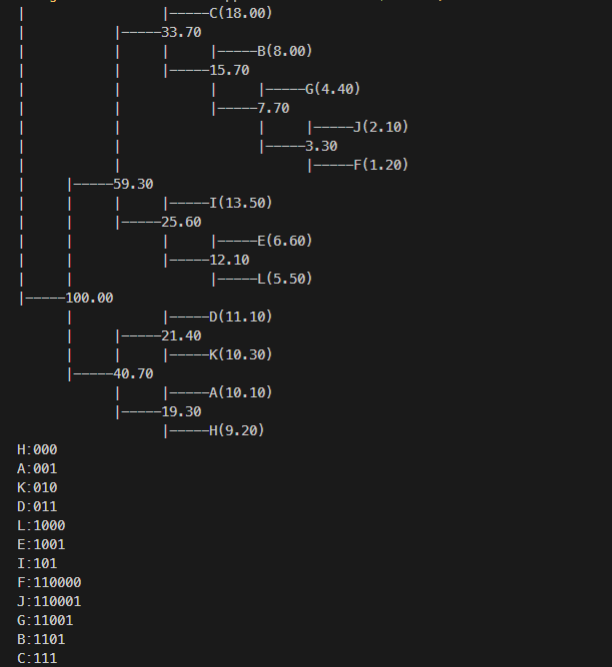
\includegraphics[width=12cm]{img/lab5/lab5.png}
    \label{fig:my_label}
\end{figure}



\subsection{3-SUM问题}

给定 A,B,C 三个数组(长度依次为 $n, m, p$),求出所有满足 $A[i] + B[j] = C[k]$ 的组合,并按照 $A[i], B[j], C[k]$ 的顺序保存每一组值。

下面的代码提供了一种时间复杂度为 $O(nmp)$ 的暴力方法:

\begin{lstlisting}
    vector<vector<int>> three_sum_brute_force(vector<int> A, vector<int> B, vector<int> C) {
        vector<vector<int>> res;
        for(int i = 0; i < A.size(); i++) {
          for(int j = 0; j < B.size(); j++) {
            for(int k = 0; k < C.size(); k++) {
              if(C[k] == A[i] + B[j]) {
                vector<int> temp = {A[i], B[j], C[k]};
                res.push_back(temp);
              }
            }
          }
        }
        return res;
    }
\end{lstlisting}

现在需要你利用贪心思想进行优化。

\begin{lstlisting}
    vector<vector<int>> three_sum(vector<int>& A, vector<int>& B, vector<int> &C) {
        // 请在这里完成你的代码
    }
\end{lstlisting}

\textbf{提示:} 首先将 $A,B$ 进行排序,然后对于每一个 $C[k]$,利用 A 和 B 的单调性快速找到所有满足条件的 $A[i], B[j]$。


\textbf{数据范围:}
\begin{itemize}[noitemsep]
    \item 70\% 的数据满足:$1\le n, m, p \le 300$
    \item 100\% 的数据满足:$1\le n, m, p \le 1000$,保证 A 和 B 中所有的元素都不重复出现
\end{itemize}



\section{实验思考}

\begin{enumerate}
    \item Huffman 树在构建过程中,选择的节点左右顺序可以调换吗,为什么?
    \item 3-SUM 问题中,你的优化方法时间复杂度是多少?
    \item 3-SUM 问题中,如果 A,B 数组中存在重复元素,那么原来的解法是否依旧有效,为什么?
\end{enumerate}

\section{拓展实验(仅供参考,实际以OJ上为准)}

\subsection{分发蛋糕I}
六一儿童节快到了,作为老师的你想要给班里的孩子们分发一些蛋糕,但是考虑到经费问题,每个孩子最多只能分到一个蛋糕。

班里面共有 $n$ 个孩子,第 $i$ 个孩子的胃口值是 $g[i]$。你提前买到了 $m$ 个蛋糕,第 $j$ 个蛋糕的尺寸是 $s[j]$。第 $i$ 个孩子感到满足的条件是他分配到的蛋糕尺寸大于等于他的胃口值,即 $s[j] >= g[i]$。你能找到一种合理分配蛋糕的方案使得感到满足的孩子数量最多吗?请输出这个数量。

数据范围:$1\le n, m \le 1*10^5, 1\le g[i], s[j] \le 10^9$。

\begin{itemize} [noitemsep]
    \item 示例一
          \begin{itemize}[noitemsep]
              \item[] 输入: g = [1, 2, 3], s = [1, 1]
              \item[] 输出: 1
          \end{itemize}
    \item 示例一
          \begin{itemize}[noitemsep]
              \item[] 输入: g = [1, 2], s = [1, 2, 3]
              \item[] 输出: 2
          \end{itemize}
\end{itemize}

\subsection{分发蛋糕II}

六一儿童节快到了,作为老师的你想要给班里的孩子们分发一些蛋糕,但是考虑到经费问题,每个孩子最多只能分到一个蛋糕。

在本题中,每个孩子的胃口值是一个区间 $g[i][0]\sim g[i][1]$,只有他收到的蛋糕尺寸 $x$ 满足 $g[i][0] \le x \le g[i][1]$ 时,才会感到满足。现在老师买了 $m$ 种蛋糕,第 $j$ 种蛋糕的尺寸为 $s[j][0]$,共买了 $s[j][1]$ 个。

你能找到一种合理分配蛋糕的方案使得感到满足的孩子数量最多吗?请输出这个数量。

数据范围:$1\le n, m \le 2500, 1\le g[i][0], g[i][1], s[j][0], s[j][1] \le 1000$。

\begin{itemize} [noitemsep]
    \item 示例
          \begin{itemize}[noitemsep]
              \item[] 输入: g = [[3, 10], [2, 5], [1, 5]], s = [[6, 2], [4, 1]]
              \item[] 输出: 2
              \item[] \small 解释:第一种蛋糕尺寸为 6,个数为 2。但仅能满足第一个孩子([3, 10]),第二种蛋糕尺寸为 4,个数为 1,仅能满足第二个孩子([2, 5])或第三个孩子([1,5])。
          \end{itemize}
\end{itemize}


\textbf{请注意本题算法时间复杂度最大应为 $O(nm + n\log n + m\log m)$}

\subsection{洪水泛滥}

镇子里洪水泛滥,Farmer John和他力大无穷的奶牛们准备出发解决这个问题。

镇子里有$n$个地点,对于第$i$个地点,$s_i$为他们消除洪水需要的力气,$f_i \space (f_i \in \{0, 1\})$为Farmer John对地形的适应度,$c_i \space (c_i \in \{0, 1\})$为奶牛对地形的适应度。$f_i$为1代表Farmer John适应该地点,否则不适应,奶牛同理。

他们想先选出一部分地点解决问题,同时,如果太过不适应会影响他们的发挥,所以他们适应的地点数都不能低于$a$,在这种情况下,他们想消耗尽可能少的力气($w$)。

请你找出这些地点。

数据范围:$1 \leq a \leq n \leq 2 \times 10^{5},1 \leq s_i \leq 10^4,f_i \in \{0, 1\},c_i \in \{0, 1\}$。

\begin{itemize} [noitemsep]
    \item 示例
          \begin{itemize}[noitemsep]
              \item[] 输入: n=5,a=2,[$s_i$ $f_i$ $c_i$]=[[6 0 0],[9 0 0],[1 0 1],[2 1 1],[5 1 0]]
              \item[] 输出: w=8
          \end{itemize}
\end{itemize}

\subsection{高效机械}

你有一些机器人一列排开,间隔$1$个单位长度,每个机器人最多只能承载$w$单位重量。

狡猾的合作商趁你不注意,在你的机器人列上放置了$s$块钢板,第$i$块钢板的起始位置是机器人$a_i$,长度为$b_i - a_i$,每$1$长度的钢板重量为$1$个单位。

这样下去你的机器人很快因为高负载而停止工作,请你拿走尽可能少($n$)的钢板,使得所有机器人都不处于过载的状态。

数据范围:$1\leq s \leq w \leq 200,1 \leq a_i \leq b_i \leq 200$,$1\leq k_i \leq s$。

\begin{itemize} [noitemsep]
    \item 示例
          \begin{itemize}[noitemsep]
              \item[] 输入: s=7,w=2,[$a_i$ $b_i$]=[[11 11],[9 11],[7 8],[8 9],[7 8],[9 11],[7 9]]
              \item[] 输出: n=3,$k_i$=[1,4,7]
          \end{itemize}
\end{itemize}


\section{附录}

\subsection{sort}

C++ STL 提供了 sort 函数,可以方便的对数据进行排序,它包含在 algorithm 头文件中:

\begin{lstlisting}
        vector<int> a = {10, 1, 5, 7, 2};
        sort(a.begin(), a.end()); // 对 a 中元素进行排序
\end{lstlisting}

它默认从小到大排序,如果你想从大到小排,可以这样写:
\begin{lstlisting}
        bool cmp(int x, int y) {
            return x > y;
        }
        int main(){
            vector<int> a = {10, 1, 5, 7, 2};
            sort(a.begin(), a.end(), cmp); // 对 a 中元素进行排序
        }
\end{lstlisting}

同样,如果是一个结构体,你也可以用 cmp 来完成排序规则的指定:
\begin{lstlisting}
        struct rec {
            int x, y;
            rec(int x, int y):x(x),y(y){}
        };
        bool cmp(rec &lth, rec &rth) {
            return lth.x == rth.x ? lth.y < rth.y : lth.x < rth.x;
        }
        int main(){
            vector<rec> a = {{1, 3}, {1, 2}, {2, 3}};
            sort(a.begin(), a.end(), cmp); // 对 a 中元素进行排序
        }
\end{lstlisting}

对于拓展题 II,可能会用到关于 vector 的排序:

\begin{lstlisting}
        bool cmp(vector<int> &lth, vector<int> &rth) {
            return lth[0] == rth[0] ? lth[1] < rth[1] : lth[0] < rth[0];
        }
        int main(){
            vector<vector<int>> a = {{5, 10}, {4, 5}, {3, 8}, {4, 3}};
            sort(a.begin(), a.end(), cmp);
            for(auto &v : a) {
                cout << v[0] << ' ' << v[1] << endl;
            }
        }
\end{lstlisting}

排序后顺序为:[3, 8], [4, 3], [4, 5], [5, 10]

\subsection{priority\_queue}
priority\_queue 是 C++ STL 中的优先队列,遵循 "First in, Largest out" 原则。它内部实现基于二叉堆,可以像二叉堆一样完成元素的存取。

下面展示了一些优先队列的用法:

\begin{lstlisting}
        #include <iostream>
        #include <queue> // priority_queue 包含在 queue 头文件中
        
        using namespace std;
        
        int main() {
            priority_queue<int> q; // 构建一个大顶堆
            q.push(3);  // 将元素压入堆中
            q.push(1);
            q.push(4);
            q.push(2);
            while(q.size()) { // 或者写成 !q.empty()
                cout << q.top() << ' ';
                q.pop(); // 堆顶弹出
            }
            return 0;
        }
\end{lstlisting}

上述代码的输出结果是 4 3 2 1 。

如果要使用小顶堆,你可以这样做:

\begin{lstlisting}
        priority_queue<int, vector<int>, greater<int>> q;
\end{lstlisting}

其中包含三个模版参数,第一个 int 表示队内元素类型是 int,第二个 vector<int> 表示内部的二叉堆是基于 vector<int> 实现的,第三个参数表示元素排序时采用 greater<int> 规则。

由于内部排序时默认使用的是 less<int> 规则,数组按照从小到大排序,优先队列会优先选取后面的元素放在堆顶,所以当排序规则采用 greater<int>时,数组将从大到小排序,优先队列仍然优先选取后面的元素即较小的元素放在堆顶,这样就构造出了一个最小堆。

如果堆中的元素是自定义结构体,没有提供像 less 和 greater 这样的比较函数时,我们就需要
自定义一个满足需求的排序规则。比如在 Huffman 编码中我们需要对 TreeNode* 自定义排序规则:

\begin{lstlisting}
        struct TreeNode {
            char symbol;       // 编码的字母
            double freq;       // 对应的频率
            TreeNode *left;    // 左孩子
            TreeNode *right;   // 右孩子
            // 构造函数
            TreeNode()
                : symbol('\0'), freq(0), left(NULL), right(NULL) {}
            // 用symbol和freq构造 TreeNode 对象
            TreeNode(char symbol_, double freq_)
                : symbol(symbol_), freq(freq_), left(NULL), right(NULL) {}
            // () 函数,用于规定优先队列比较运算
            bool operator () (const TreeNode* lhs, const TreeNode* rhs) {
                return lhs->freq > rhs->freq;
            }
        };
        priority_queue<TreeNode*, vector<TreeNode*>, TreeNode> q;
\end{lstlisting}

\section*{更新历史}

\begin{center}
    \begin{tabular}{|c|c|c|}
        \hline
        \textbf{更新时间} & \textbf{助教} & \textbf{更新内容} \\
        \hline
        2024 & 黄韦杰, 刘嘉杰 & 修改与添加拓展题描述\\
        2023 & 王梓健, 黄韦杰 & 添加 OJ 相关表述,完善本地环境使用方法 \\
        2022 & 邢广杰, 李晓晓 & 完善实验题目,开始更新记录 \\
        2021 & 韩耀东 & 主要内容构建 \\
        % Add more rows as needed
        \hline
        \end{tabular}
\end{center}

\end{document}